% VUT FIT MITAI
% MSZ 2021/2022
% Author: Vladimir Dusek
% Login: xdusek27

%%%%%%%%%%%%%%%%%%%%%%%%%%%%%%%%%%%%%%%%%%%%%%%%%%%%%%%%%%%%%%%%%%%%%%%%%%%%%%%%

% Path to figures
\graphicspath{{pds/detekce_sitovych_incidentu/figures}}

%%%%%%%%%%%%%%%%%%%%%%%%%%%%%%%%%%%%%%%%%%%%%%%%%%%%%%%%%%%%%%%%%%%%%%%%%%%%%%%%

\chapter{PDS~--~Metody detekce síťových incidentů (signatury, statistické metody) a nástroje (IDS/IPS).}

%%%%%%%%%%%%%%%%%%%%%%%%%%%%%%%%%%%%%%%%%%%%%%%%%%%%%%%%%%%%%%%%%%%%%%%%%%%%%%%%

\section{Metadata}

\begin{compactitem}
    \item Předmět: Přenos dat, počítačové sítě a protokoly (PDS)
    \item Přednáška:
    \begin{compactitem}
        \item \path{07-ids.pdf}
    \end{compactitem}
    \item Záznam:
    \begin{compactitem}
        \item 2021-03-26
    \end{compactitem}
\end{compactitem}

\begin{compactitem}
    \item Předmět: Návrh, správa a bezpečnost (NSB)
    \item Přednáška:
    \begin{compactitem}
        \item \path{03-IDS.pdf}
    \end{compactitem}
    \item Záznam:
    \begin{compactitem}
        \item 2021-02-23
    \end{compactitem}
\end{compactitem}

%%%%%%%%%%%%%%%%%%%%%%%%%%%%%%%%%%%%%%%%%%%%%%%%%%%%%%%%%%%%%%%%%%%%%%%%%%%%%%%%

\section{Úvod a kontext}

\paragraph*{Identifikace a monitorování síťového provozu} \begin{compactitem}
    \item Co je cílem? \begin{compactitem}
        \item Identifikace protokolu (na různých vrstvách).
        \item Identifikace aplikace.
        \item Pokud je identifikován nedovolený provoz, tak kontaktovat správce.
    \end{compactitem}
    \item Proč to dělat? \begin{compactitem}
        \item Bezpečnost~--~Detekce útoků a nedovoleného chování.
        \item Diagnostika~--~Správné chování systémových i uživatelských aplikací.
        \item Rozlišení služeb~--~Nastavení kvality služeb, prioritizace kritických přenosů.
        \item Vytížení sítě~--~Sledování rozložení sítě, vytížení síťových prvků a služeb.
        \item Účtování služeb~--~Identifikace provozu VoIP, IPTV, apod.
    \end{compactitem}
\end{compactitem}

\paragraph*{Síťový tok} Jednosměrná posloupnost paketů, identifikovaná zdrojovou IP adresou, zdrojovým portem, cílovou IP adresou a cílovým protem.

\paragraph*{Síťové tunelování} Technika, která pro přenos síťového spojení používá jiné síťové spojení (Zapouzdření komunikace do jiného protokolu.). Umožňuje: přenášet data přes nekompatibilní sítě; obcházet administrativní omezení určité sítě; poskytovat zabezpečenou komunikaci přes nezabezpečenou, resp. nedůvěryhodnou síť.

%%%%%%%%%%%%%%%%%%%%%%%%%%%%%%%%%%%%%%%%%%%%%%%%%%%%%%%%%%%%%%%%%%%%%%%%%%%%%%%%

\section{Nástroje IDS/IPS}

\paragraph*{Intrusion Detection System (IDS)} Identifikovat provoz a v případě, že se jedná nedovolený provoz, tak informovat správce. Ten rozhodne, jaké budou kroky (zda se zablokuje, nebo zda se jedná o falešnou pozitivitu).

\paragraph*{Intrusion Prevention System (IPS)} Detekovat provoz a v případě, že se jedná nedovolený provoz, tak ho zablokovat. Nebezpečné v případě falešné pozitivity. Můžeme odřiznout provoz, který považujeme za nedovolený, ale ve skutečnosti se jedná o provoz, který jsme nečekali. Většinou se v praxi volí IDS.

\paragraph*{Síťový incident} Identifikace nedovoleného provozu.

%%%%%%%%%%%%%%%%%%%%%%%%%%%%%%%%%%%%%%%%%%%%%%%%%%%%%%%%%%%%%%%%%%%%%%%%%%%%%%%%

\section{Identifikace provozu pomocí hodnot z hlaviček paketů}

\begin{compactitem}
    \item Využití informací z hlaviček jednotlivých protokolů TCP/IP. Jaké informace lze využít? \begin{compactitem}
        \item Na linkové vrstvě (L2): \begin{compactitem}
            \item Field \path{EtherType}~--~IPv4, IPv6, ARP, RARP, autentizace 802.1x, \dots
        \end{compactitem}
        \item Na síťové vrstvě (L3): \begin{compactitem}
            \item Field \path{protocol}~--~IPv6 nad IPv4, ICMP, IGMP, transportní protokoly (UDP, TCP, SCTP, \dots), směrovací protokoly (EIGRP, ESPF, \dots), multicast (PIM), \dots
        \end{compactitem}
        \item  Na transportní vrstvě (L4): \begin{compactitem}
            \item Field \path{Source Port}, \path{Destination Port}, rozpoznání služby na základě portu~--~FTP, SSH, Telnet, SMTP, DNS, DHCP, HTTP, POP3, NTP, IMAP, SNMP, LDAP, HTTPS, \dots
        \end{compactitem}
        \item  Na aplikační vrstvě vrstvě (L7): \begin{compactitem}
            \item Specifické pro aplikace (např: pro HTTP rozpoznávání jednotlivých metod).
        \end{compactitem}
    \end{compactitem}
    \item Rychlé, dobře implementovatelné a univerzální řešení. Má své limity: \begin{compactitem}
        \item Aplikace nemusí být pevně svázána s portem (dynamické porty).
        \item Tunelování, šifrování (spoustu věcí je zapouzdřováno do SSL/TLS), VPN.
        \item IPv6 nad IPv4.
        \item Skryté kanály~--~Tunelování skrze protokoly, kde se neočekává nic nelegitimního, běžně se nefiltrují (ICMP, DNS).
    \end{compactitem}
    \item Na tomto konceptu fungují firewally.
\end{compactitem}

%%%%%%%%%%%%%%%%%%%%%%%%%%%%%%%%%%%%%%%%%%%%%%%%%%%%%%%%%%%%%%%%%%%%%%%%%%%%%%%%

\section{Identifikace provozu dle signatury}

% Clanek: http://dpnm.postech.ac.kr/papers/NOMS/08/LASER.pdf

\begin{compactitem}
    \item Signatura (pattern, signature) je statický řetězec tvořený posloupností znaků z hlavičky či těla protokolu, který slouží k rozpoznání daného protokolu. \begin{compactitem}
        \item Je to \uv{reprezentující} podřetězec paketu komunikace (paket jako řetězec bytů~--~ASCII).
        \item Určujeme až v aplikačních datech (TCP/UDP payload).
    \end{compactitem}
    \item Signatura ale může mít různou podobu: \begin{compactitem}
        \item Řetězec, který se vyskytuje na začátku, resp. na nějakém fixním offsetu payloadu.
        \item Řetězec, který se vyskytuje na různém místě v payloadu.
        \item Posloupnost podřetězců, která se vyskytuje v payloadu.
    \end{compactitem}
    \item Pokud se snažíme identifikovat provoz na základě signatury, tak typicky signaturu nehledáme v celém paketu (příliš náročné), ale pouze v prvních X bytech payloadu.
    \item Signatura v paketu vs. toku \begin{compactitem}
        \item Jednoduchá možnost~--~Signatura pouze na základě informací v paketu.
        \item Složitější možnost~--~Signatury napříč pakety (v datovém toku). \begin{compactitem}
            \item Příklad: signaturu pro identifikaci TLS provozu, by mohla mít podobu dvou řetězců, které se vyskytují každý v jiném paketu (1~--~\uv{client hello}, 2~--~\uv{server hello}).
        \end{compactitem}
    \end{compactitem}
    \item S novou verzí protokolu, je většinou třeba aktualizovat signaturu, protože se změnila struktura komunikace.
    \item Lze vytvořit manuálně na základě specifikace protokolu a nebo automatizovat (\textit{Longest common subsequence problem}).
    \item Použití: Někde poslouchám síťový provoz a mám databázi signatur. Snažím se najít v toku signaturu z databáze a tím identifikovat aplikaci.
\end{compactitem}

% http://l7-filter.sourceforge.net/protocols

\noindent\begin{minipage}{\linewidth}
    \begin{lstlisting}[language=Python, caption={Příklad signatury pro detekci IRC. Pomocí regulárního výrazu je specifikována kostra řetězce.}]
# First thing that happens is that the client sends NICK and USER, in
# either order.  This allows MIRC color codes (\x02-\x0d instead of
# \x09-\x0d).
^(nick[\x09-\x0d -~]*user[\x09-\x0d -~]*:|user[\x09-\x0d -~]*:[\x02-\x0d -~]
*nick[\x09-\x0d -~]*\x0d\x0a)
\end{lstlisting}
\end{minipage}

\noindent\begin{minipage}{\linewidth}
    \begin{lstlisting}[language=Python, caption={Příklad signatury pro detekci BitTorrentu. Signatura je založená na klíčových slovech.}]
^(\x13bittorrent protocol|azver\x01$|get /scrape\?info_hash=get
/announce\?info_hash=|get /client/bitcomet/|GET /data\?fid=)
|d1:ad2:id20:|\x08'7P\)[RP]
\end{lstlisting}
\end{minipage}

\noindent\begin{minipage}{\linewidth}
    \begin{lstlisting}[language=Python, caption={Příklad signatury pro detekci SSL provozu. Detekce Client Hello paketu, kdy se vyměňují informace o šifrování.}]
// SSL Hello with certificate, Client Hello
^(.?.?\x16\x03.*\x16\x03|.?.?\x01\x03\x01?.*\x0b)
\end{lstlisting}
\end{minipage}

\subsection*{Automatizace vytváření signatur}

\begin{compactitem}
    \item Algoritmus LCS (Longest Common Subsequence).
    \item Algoritmus hledá \uv{nejbližší} společný řětězec v toku (algoritmus definuje metriku blízkosti).
    \item Proces vytvoření signatury: \begin{compactitem}
        \item Odchytím si typickou komunikaci aplikace, kterou chci identifikovat v provozu~--~Několik toků, které jsou dostatečně reprezentativní.
        \item Z každého toku vezmeme X prvotních paketů (např. 10 stačí).
        \item Poté iterativně hledám \uv{nejbližší} společný podřetězec vždy pro dvojici toků (kandidát).
        \item Cyklus končí, až se kandidát přestane měnit. Výsledek je signatura (minimální možná délka, 2 znaky jsou málo).
    \end{compactitem}
\end{compactitem}

%%%%%%%%%%%%%%%%%%%%%%%%%%%%%%%%%%%%%%%%%%%%%%%%%%%%%%%%%%%%%%%%%%%%%%%%%%%%%%%%

\section{Identifikace provozu dle statistického chování}

\begin{compactitem}
    \item Vytvoření statistického modelu protokolu na základě trénovacích dat. \begin{compactitem}
        \item Popis chování na základě metadat o provozu (odezva, velikost paketu, počet paketů v daném směru, \dots).
        \item Zkoumáme prvních $n$ bytů toku, které jsou spíše specifické pro protokol (navazování spojení).
        \item Na rozdíl od signatur se nezkoumá obsah hlaviček a těla protokolu, ale pouze statistické vlastnosti jeho chování.
    \end{compactitem}
    \item
    \item Klasifikace neznámého protokolu: Vybereme model s nejlepší vzdáleností od neznámého protokolu.
    \item Vytváření se tzv. \textbf{otisk protokolu} (\textit{fingerprint})~--~soubor vlastností (chování) protokolu, které lze využít k jednoznačné identifikaci protokolu.
\end{compactitem}

\subsection*{Metoda jednoduchých statistických otisků}

\begin{compactitem}
    \item Trénovací data: mějme $n$ síťových toků. Z prvních $m$ paketů každého toku se extrahuje: \begin{compactitem}
        \item velikost paketu;
        \item časový odstup paketů (závisí na tom co dělá klient a co dělá server);
        \item pořadí paketů v toku.
    \end{compactitem}
    \item Učení: \begin{compactitem}
        \item Z trénovacích dat se modeluje statistické chování každého paketu v toku. Např. velikost prvního paketu odpovídá tomuhle pravděpodobnostnímu rozdělení, časový odstup druhého paketu od prvnímu odpovídá jinému pravděpodobnostnímu rozdělení. (Typicky normální rozdělení).
        \item Poté se aplikují gaussovské filtry pro odstranění šumu.
        \item Vzniká tzv. \uv{maska} a je určena nějaká prahová hodnota (na základě \textit{anomaly score}, která se spočítá z vektoru anomálií).
    \end{compactitem}
    \item Model: protokol je reprezentován otiskem (\textit{fingerprint})~--~\uv{maska}, prahová hodnota
    \item Klasifikace: \begin{compactitem}
        \item Máme neznámý tok, který chceme klasifikovat.
        \item Sleduju velikosti paketů, odstupy paketů a na základě toho spočítám \textit{anomaly score} pro tok.
        \item Získané \textit{anomaly score} porovnám s prahovou hodnotou.
    \end{compactitem}
\end{compactitem}

\begin{figure}[H]
    \centering
    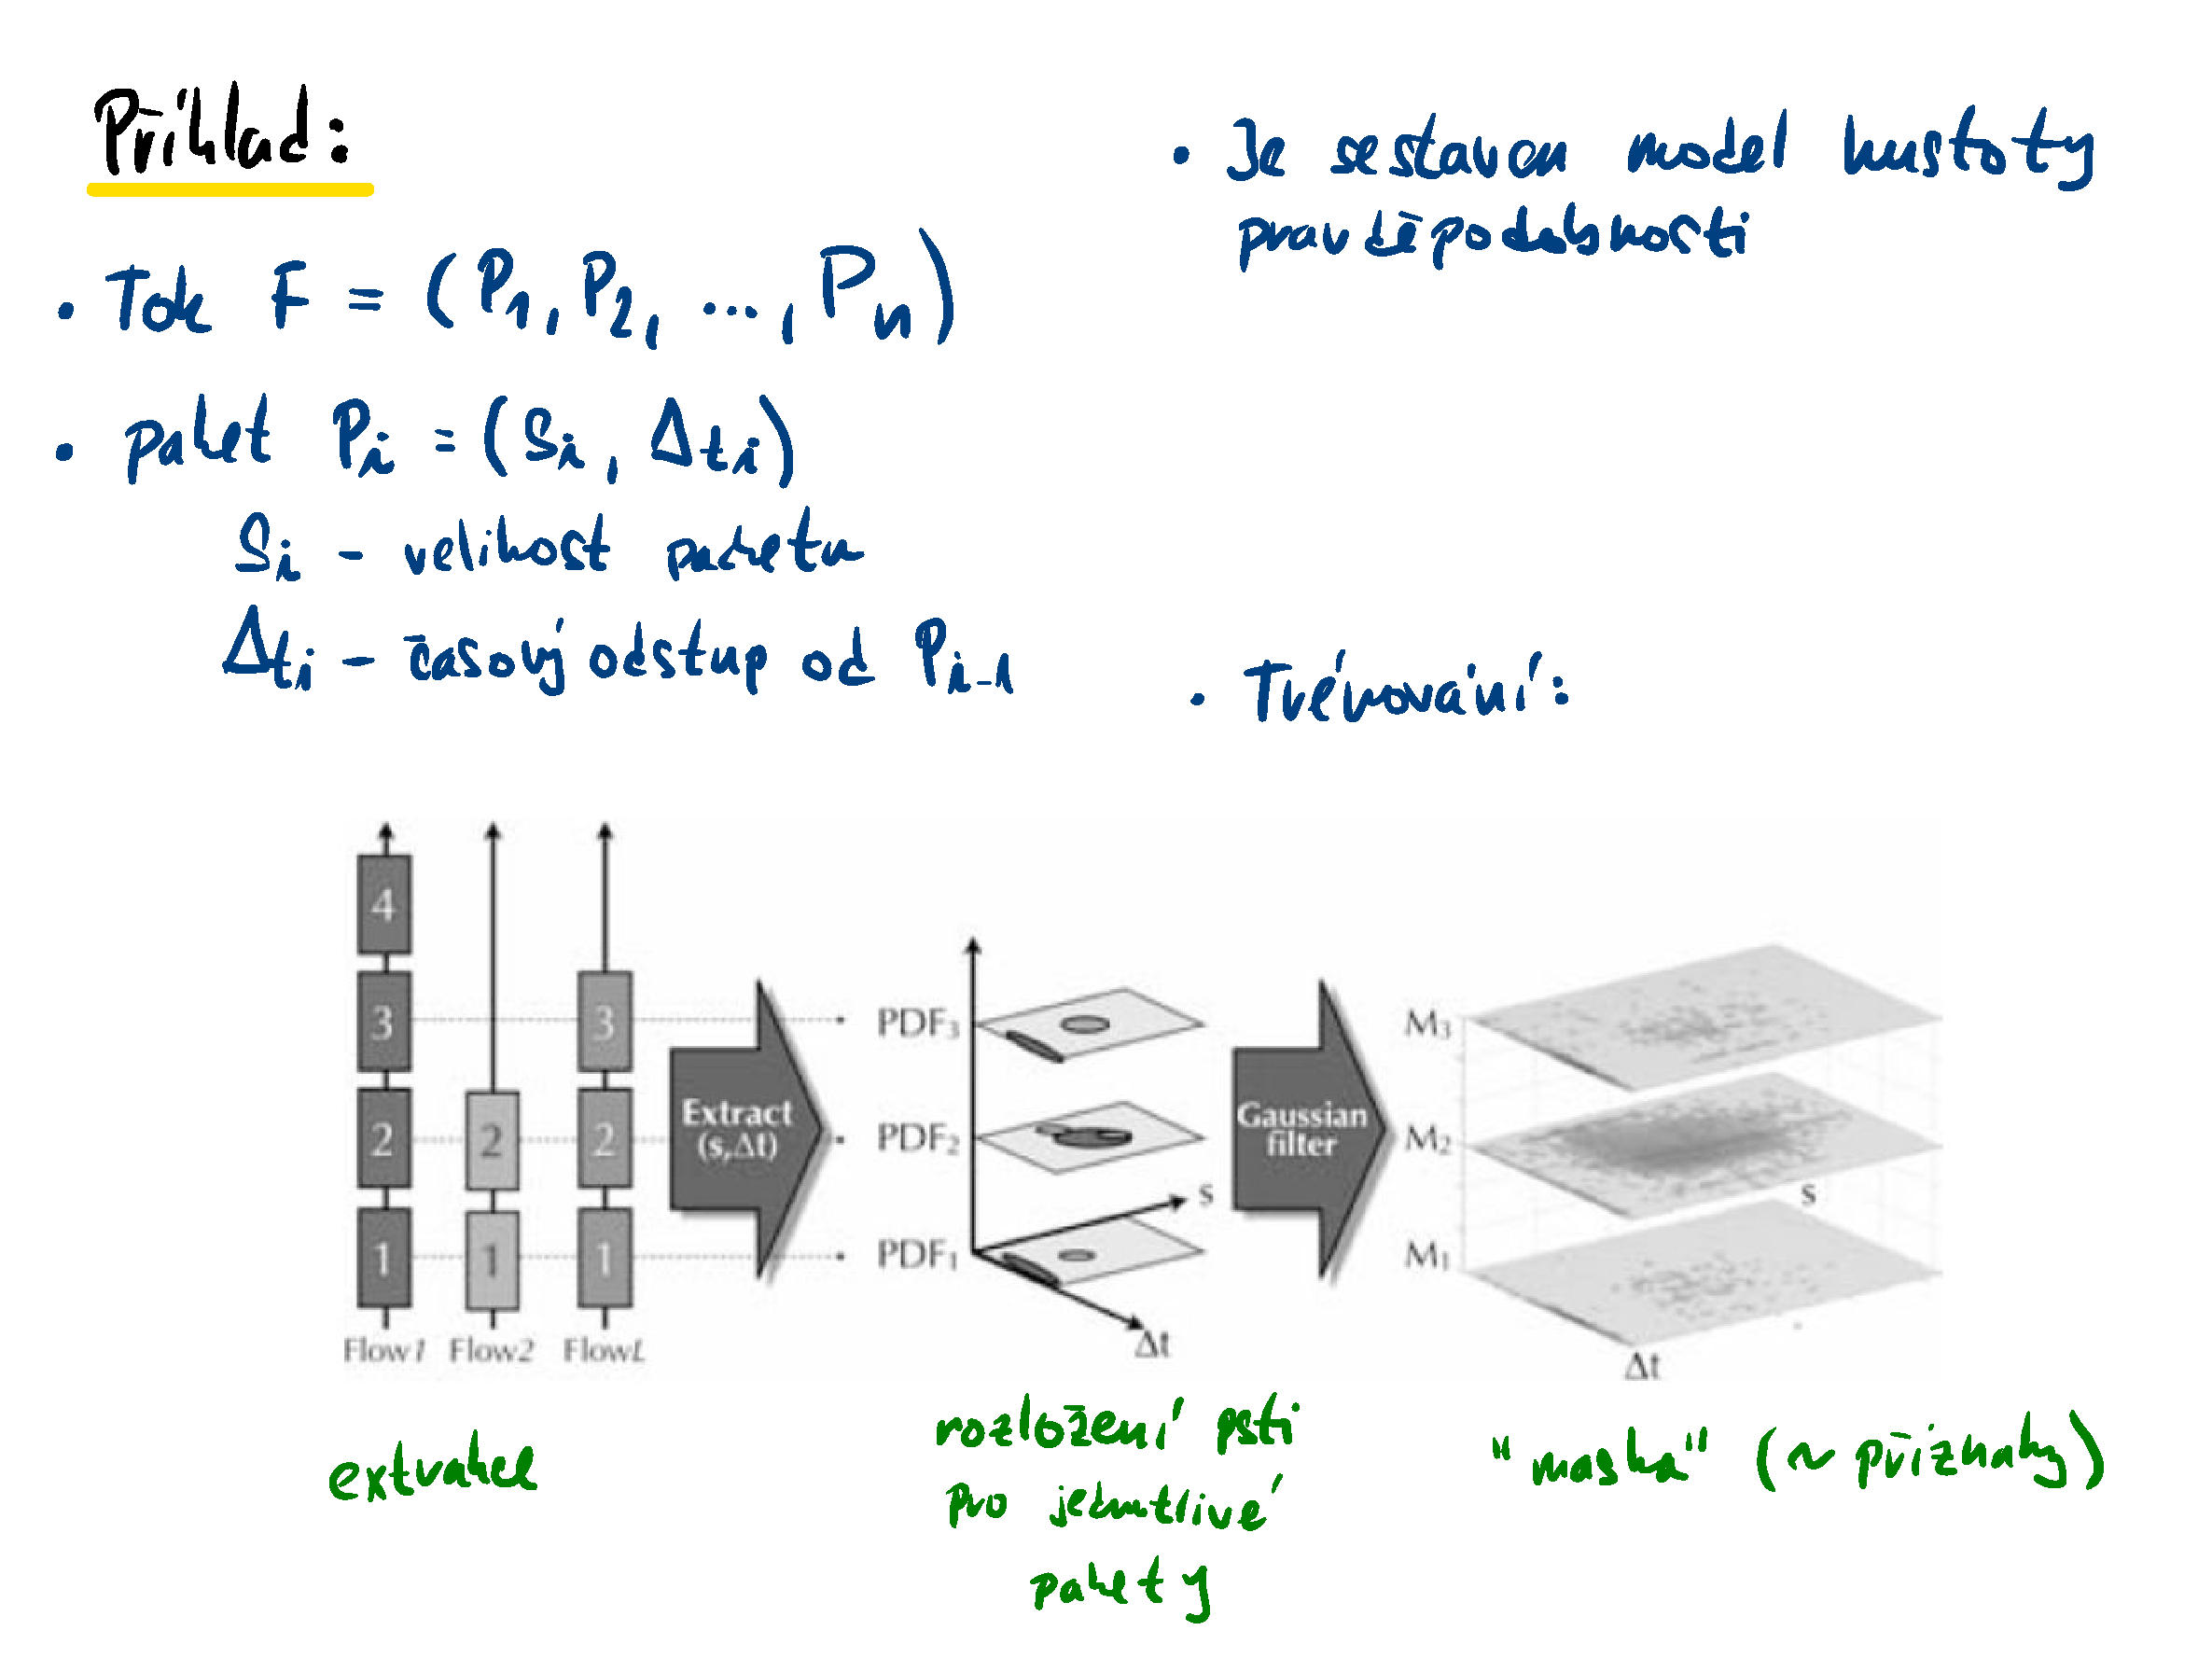
\includegraphics[width=1\linewidth]{metoda_jednoduchych_statistickych_otisku_priklad.pdf}
    \caption{Princip metody jednoduchých statistických otisků~--~fáze učení.}
\end{figure}

\subsection*{Statistical Protocol IDentification (SPID)}

\begin{compactitem}
    \item Kombinuje statistické chování s atributy.
    \item Statistické atributy: směr paketů, pořadí paketů, velikost paketů.
    \item Aplikační atributy: četnost konkrétních bytů, hodnota off-setu.
    \item Model protokolu používá pro klasifikaci pravděpodobnostní vektory atributů.
    \item Pro porovnání měří odlišnost dvou pravděpodobnostních rozložení.
    \item Příklad jaké atributy přenosu lze použít pro rozlišení aplikačního protokolu. \begin{compactitem}
        \item Bytová frekvence prvního paketu TCP v každém směru (myšlenka: obsah je typický, pouze pro začátek toho toku~--~navázání spojení).
        \item Počet změn komunikace (klient $\rightarrow$ server, server $\rightarrow$ klient).
        \item Počet přenesených bytů v daném směru (RTP~--~balanced, HTTP~--~download, SMTP~--~upload).
    \end{compactitem}
\end{compactitem}

%%%%%%%%%%%%%%%%%%%%%%%%%%%%%%%%%%%%%%%%%%%%%%%%%%%%%%%%%%%%%%%%%%%%%%%%%%%%%%%%

\section{Detekce anomálie}

\begin{compactitem}
    \item Protokol jsme již identifikovali a nyní sledujeme jeho chování.
    \item Anomálie v provozu~--~odchylka komunikace od standardního (typického) provozu.
    \item Jaké anomálie mohou nastat: \begin{compactitem}
        \item Neočekávaný nárůst provozu.
        \item Snížení provozu, chybějící linky~--~Výpadek linky.
        \item Změna struktury provozu~--~Jeden uzel se snaží komunikovat se všemi v síti (sledování, detekce malwaru).
    \end{compactitem}
    \item Vytvoření modelu: \begin{compactitem}
        \item Trénovací data: typická komunikace.
        \item Natrénování modelu.
        \item Metrika pro určení odchylky od natrénovaného modelu (např. když se přesáhne práhová hodnota, vyvolá se upozornění).
    \end{compactitem}
    \item Jaké modely lze využít: \begin{compactitem}
        \item statistické modely,
        \item shlukování (k-means, k-medoids, k-nn clusters, \dots),
        \item klasifickační modely (bayesovské modely, SVM, neuronové sítě, \dots)
        \item pravděpodobnostní automaty, markovovy řetězce.
    \end{compactitem}
    \item Sbět trénovacích dat: \begin{compactitem}
        \item Netflow~--~informace o tocích (jaké IP adresy, jaké porty, jak dlouho tok trval, kolik dat se přeneslo, \dots).
        \item SNMP~--~informace o provozu (počet přenesených paketů, bytů, \dots).
        \item Úplné zachytávání paketů.
    \end{compactitem}
    \item Systém může fungovat pouze tehdy, pokud jsme schopni sestavit model běžného chování.
\end{compactitem}
